%%%%%%%%%%%%%%%%%%%%%%%%%%%%%%%%%%%%%%%%%%%%%%%%%%
%  JASA LaTeX Template File
%  To make articles using JASA.cls, Version 1.1
%  September 14, 2019
%%%%%%%%%%%%%%%%%%%%%%%%%%%%%%%%%%%%%%%%%%%%%%%%%%

%% Step 1:
%% Uncomment the style that you want to use:

%%%%%%% For Preprint
%% For manuscript, 12pt, one column style

\documentclass[reprint]{JASA}

%%%%% Preprint Options %%%%%
%% The track changes option allows you to mark changes
%% and will produce a list of changes, their line number
%% and page number at the end of the article.
%\documentclass[preprint,trackchanges]{JASA}


%% NumberedRefs is used for numbered bibliography and citations.
%% Default is Author-Year style.
%% \documentclass[preprint,NumberedRefs]{JASA}

%%%%%%% For Reprint
%% For appearance of finished article; 2 columns, 10 pt fonts

% \documentclass[reprint]{JASA}

%%%%% Reprint Options %%%%%

%% For testing to see if author has exceeded page length request, use 12pt option
%\documentclass[reprint,12pt]{JASA}


%% NumberedRefs is used for numbered bibliography and citations.
%% Default is Author-Year style.
% \documentclass[reprint,NumberedRefs]{JASA}

%% TurnOnLineNumbers
%% Make lines be numbered in reprint style:
% \documentclass[reprint,TurnOnLineNumbers]{JASA}

\usepackage{natbib}



% tightlist command for lists without linebreak
\providecommand{\tightlist}{%
  \setlength{\itemsep}{0pt}\setlength{\parskip}{0pt}}





\begin{document}
%% the square bracket argument will send term to running head in
%% preprint, or running foot in reprint style.

\title[]{Model-Based Similarity Scores for the Comparison of Cartridge
Case Impressions}

% ie
%\title[JASA/Sample JASA Article]{Sample JASA Article}

%% repeat as needed

\author{Joseph Zemmels}
% ie
%\affiliation{Department1,  University1, City, State ZipCode, Country}
\affiliation{Iowa State University}
%% for corresponding author
\email{jzemmels@iastate.edu}
%% for additional information
\thanks{other info}
\author{Heike Hofmann}
% ie
%\affiliation{Department1,  University1, City, State ZipCode, Country}
\affiliation{Iowa State University}
%% for corresponding author

%% for additional information

\author{Susan VanderPlas}
% ie
%\affiliation{Department1,  University1, City, State ZipCode, Country}
\affiliation{University of Nebraska - Lincoln}
%% for corresponding author

%% for additional information


% ie
% \author{Author Four}
% \email{author.four@university.edu}
% \thanks{Also at Another University, City, State ZipCode, Country.}

%% For preprint only,
%  optional, if you want want this message to appear in upper left corner of title page
\preprint{Zemmels, Hofmann, and VanderPlas, Statistical Analysis and
Data Mining}

%ie
%\preprint{Author, JASA}

% optional, if desired:
%\date{\today}
\date{\today}

\begin{abstract}
% Put your abstract here. Abstracts are limited to 200 words for
% regular articles and 100 words for Letters to the Editor. Please no
% personal pronouns, also please do not use the words ``new'' and/or
% ``novel'' in the abstract. An article usually includes an abstract, a
% concise summary of the work covered at length in the main body of the
% article.
Put your abstract here.
\end{abstract}

%% pacs numbers not used

\maketitle

%  End of title page for Preprint option --------------------------------- %

%% See preprint.tex/.pdf or reprint.tex/.pdf for many examples


%  Body of the article
\defcitealias{council_strengthening_2009}{NRC (2009)}
\defcitealias{pcast2016}{PCAST (2016)}

\hypertarget{introduction}{%
\section{Background \& Introduction}\label{introduction}}

A \emph{cartride case} is the part of firearm ammunition that houses the
projectile and propulsive device. When a firearm is discharged and the
projectile travels down the barrel, the cartridge case moves in the
opposite direction and slams against the back wall, the \emph{breech
face}, of the firearm. Markings on the breech face are ``stamped'' into
the surface of the cartridge case leaving so-called \emph{breech face
impressions}. In this paper, we introduce an automatic method for
measuring the similarity between two cartridge cases based on their
breech face impressions.

\hypertarget{traditional-cartridge-case-comparison}{%
\subsection{Traditional Cartridge Case
Comparison}\label{traditional-cartridge-case-comparison}}

In a traditional examination, forensic examiners use these impressions
analogous to a fingerprint to determine whether two cartridge cases were
fired from the same firearm. First, two cartridge cases are collected -
perhaps one is from a crime scene and the other is collected from a
suspect's gun. An examiner places the two cartridge cases beneath a
``comparison microscope'' that merges the views of two compound
microscopes into a single split view \citep{Thompson2017}. The examiner
assesses the ``degree of similarity'' between the markings on the
cartridge cases and reaches either an \emph{identification}, meaning the
cartridge cases were fired from the same firearm, an \emph{elimination},
meaning they were fired from different firearms, or an
\emph{inconclusive}, meaning the evidence is insufficient to make an
identification or elimination \citep{AFTE1992}.\footnote{The AFTE range
  of conclusions also permits the examiner to decide that the evidence
  is \emph{unsuitable} for examination, which can occur if evidence
  quality is poor; for example, a fragment of a cartridge case is
  recovered rather than a full cartridge case.}

Critics of traditional forensic examinations cite a lack of
``foundational validity'' underlying the procedures used by firearm and
toolmark examiners \citep{council_strengthening_2009, pcast2016}. In
particular, examiners rely largely on their subjective findings rather
than on a well-defined procedure to measure similarity.
\citetalias{pcast2016} pushed for ``developing and testing
image-analysis algorithms'' to objectively measure the similarity
between cartridge cases.

In this paper, we introduce a procedure to automatically compare digital
scans of cartridge cases. Throughout this paper, we use scans, taken by
us \textbf{{[}scientific data citation{]}}, of cartridge cases collected
by \citet{Baldwin2014}. The cartridge case scans are available as part
of the data repository at \textbf{{[}doi here{]} {[}citation{]}}. We
also provide code to reproduce the results shared in this paper at
\textbf{{[}github link here{]}}.

\hypertarget{algorithmic-cartridge-case-comparisons}{%
\subsection{Algorithmic Cartridge Case
Comparisons}\label{algorithmic-cartridge-case-comparisons}}

\hypertarget{cartridge-case-surface-scans}{%
\subsubsection{Cartridge Case Surface
Scans}\label{cartridge-case-surface-scans}}

We captured digital representations of cartridge case surfaces using
topographic scanning technology. The scanner measures the relative
surface depth and stores these measurements in a 2D array called a
\emph{surface matrix}. The left side of \autoref{fig:preProcessEffect}
depicts a surface matrix representing the region at the base of a
cartridge case surface called the \emph{primer}, which is the circular
metal cap struck by the firing pin to initiate the firing process. The
purple ring near the edges of the scan represent the boundary of the
cartridge case primer while the darker orange ring near the center of
the scan represents the deformation of metal caused by the contact with
the firing pin.

Of particular interest is the annular breech face impression region
around the firing pin impression. We isolate this region by applying a
series of manual and automatic pre-processing steps to the surface
matrix, resulting in the scan on the right side of
\autoref{fig:preProcessEffect}. The gray pixels in this image represent
structurally missing values introduced during pre-processing. See
\textbf{{[}scientific data citation{]}} for more information on the
pre-processing procedure.

\begin{figure}[htbp]
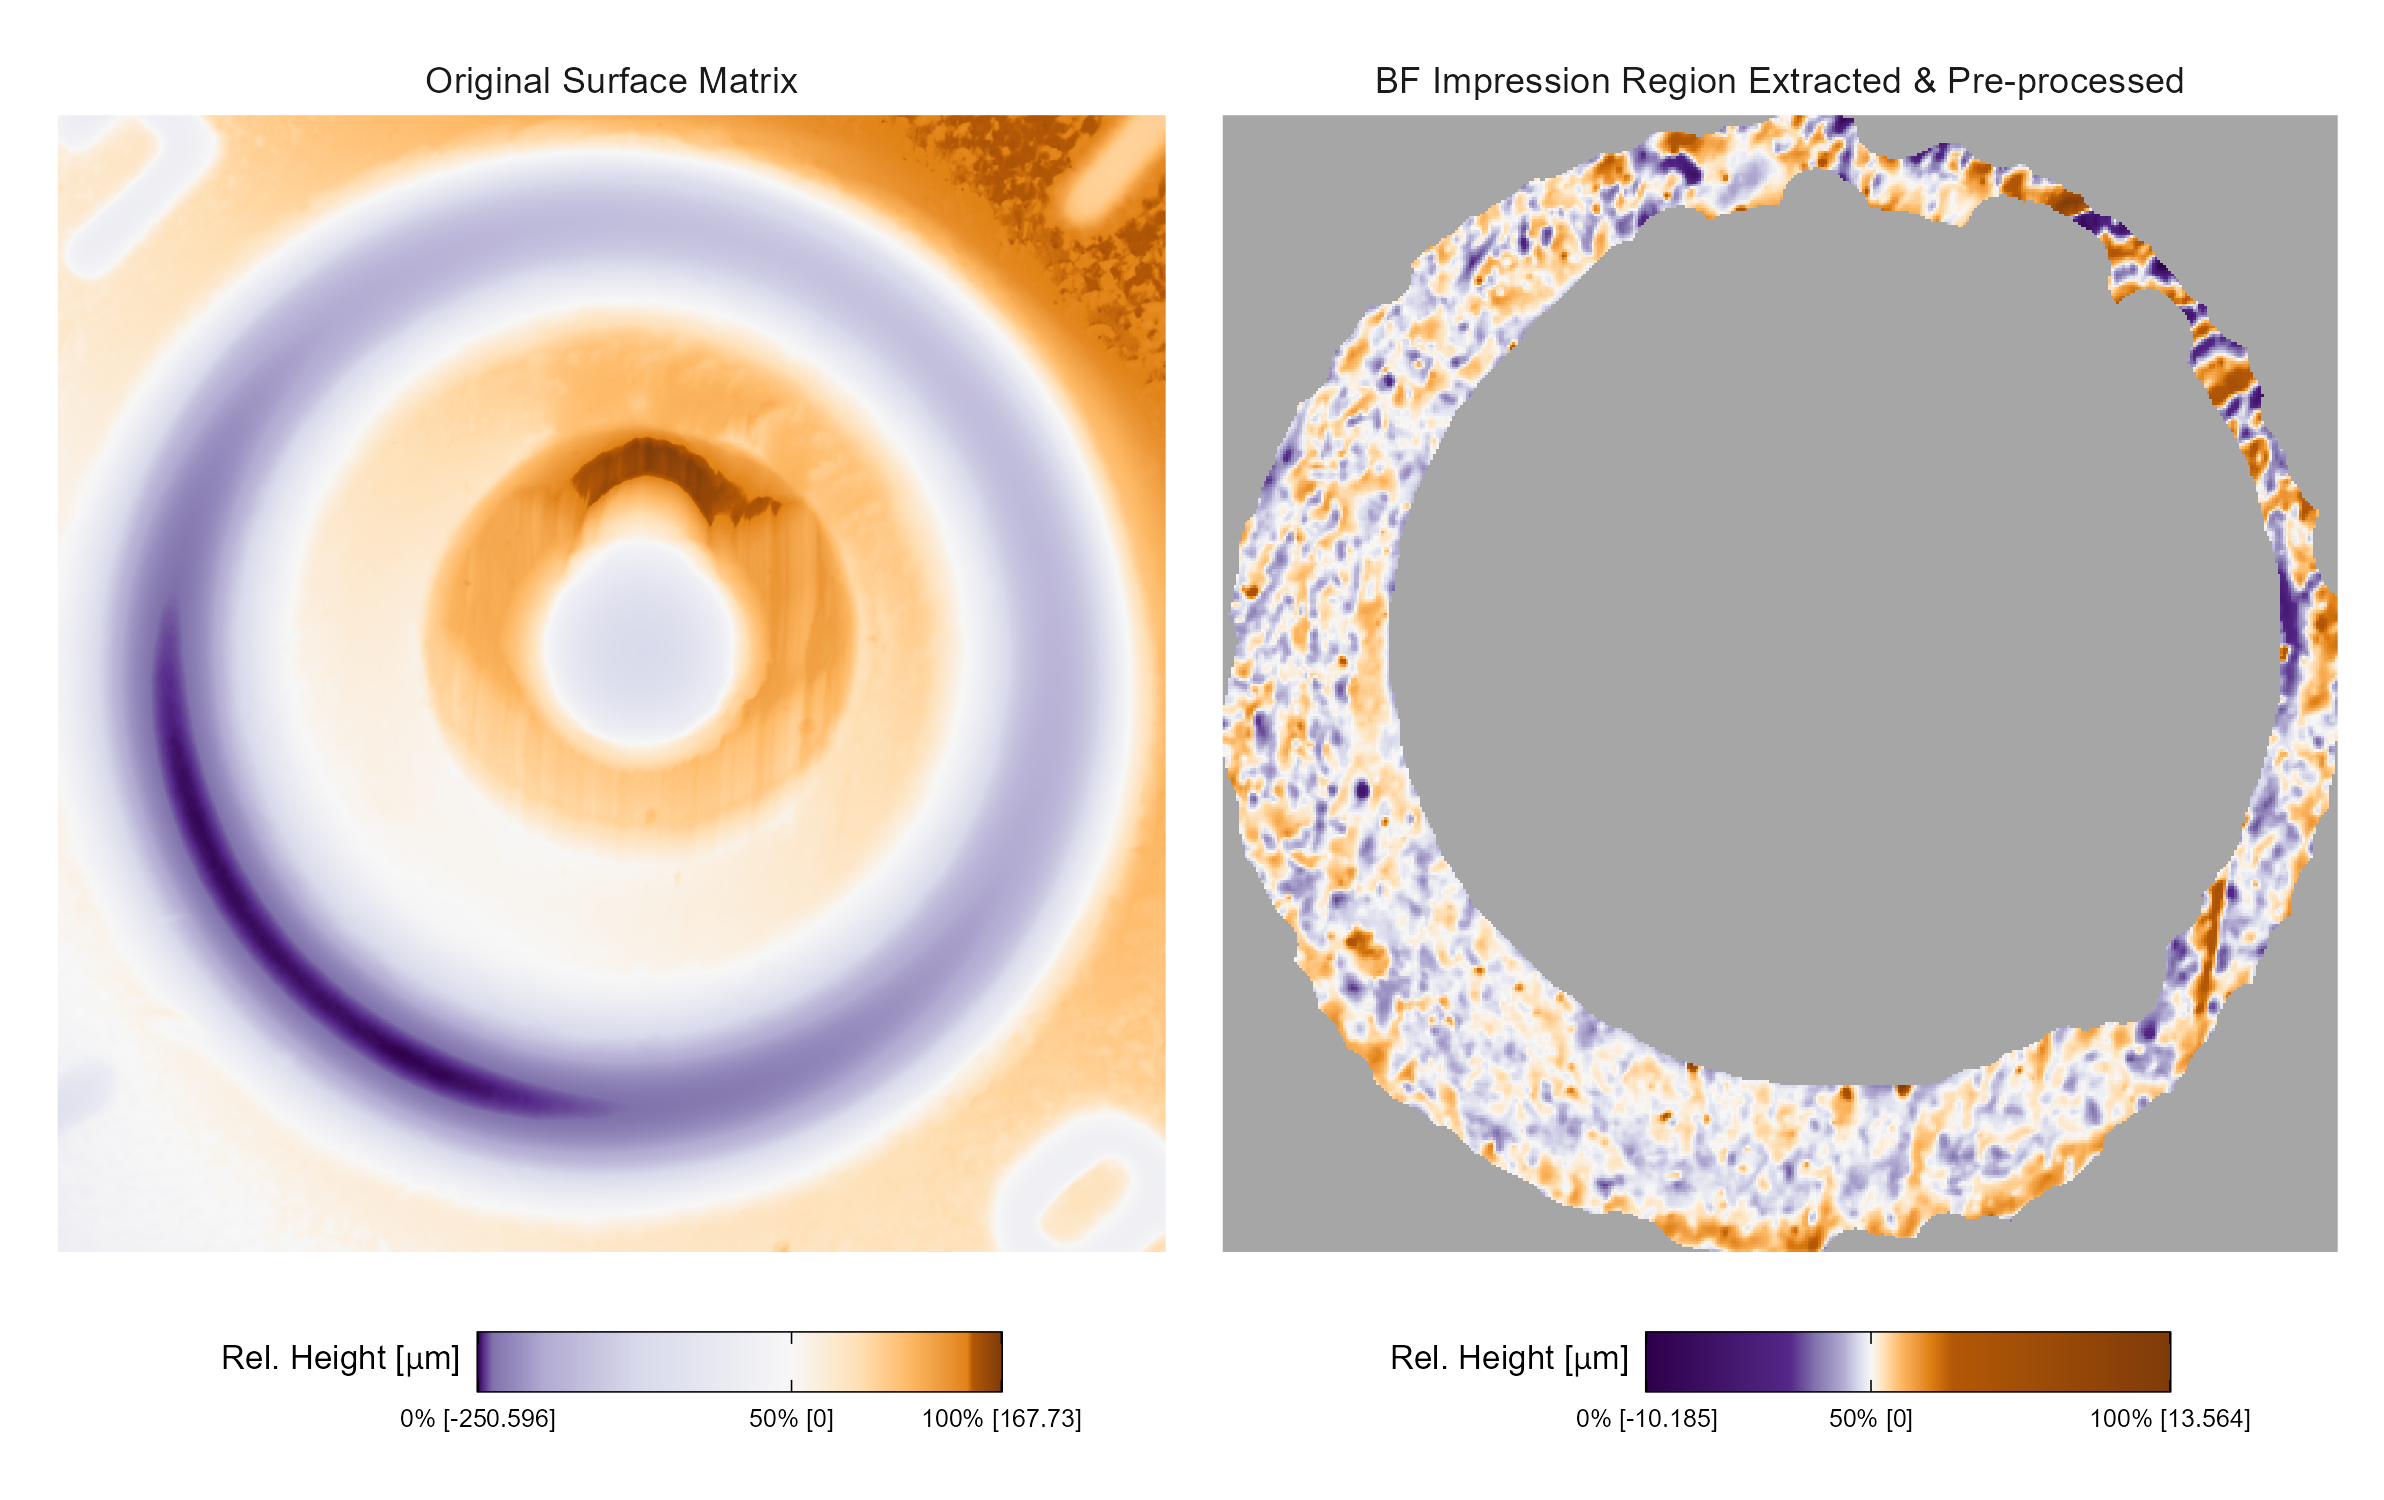
\includegraphics[width=.5\textwidth]{figures/preProcessEffect} \caption{\label{fig:preProcessEffect} We apply a sequence of pre-processing functions to each scan. Each pre-processing step further emphasizes the breech face impressions in the scan.}\label{fig:unnamed-chunk-1}
\end{figure}

Two pre-processed cartridge cases are compared to measure the similarity
of their breech face impressions. In the next section, we summarize a
technique for comparing cartridge case scans called the \emph{Congruent
Matching Cells} algorithm \citep{song_proposed_2013}.

\hypertarget{congruent-matching-cells-algorithm}{%
\subsubsection{Congruent Matching Cells
Algorithm}\label{congruent-matching-cells-algorithm}}

Recent proposals for automatic cartridge case scoring algorithms borrow
from image processing and computer vision techniques. For example,
\citet{vorburger_surface_2007} proposed using the cross-correlation
function (CCF) to compare images or scans of cartridge case surfaces.
The CCF measures the similarity between two matrices for all possible
translations of one matrix against the other. Calculating the CCF while
rotating one of the scans therefore allows for estimation of the optimal
translation and rotation, together referred to as the
\emph{registration}, between the two scans; simply choose the
rotation/translation at which the CCF is maximized.

\citet{song_proposed_2013} noted that two matching cartridge cases often
share similar impressions in specific regions, so calculating the CCF
between two full scans may not highlight their similarities. Instead,
\citet{song_proposed_2013} proposed partitioning one cartridge case scan
into a grid of ``cells'' and calculating the CCF between each cell and
the other scan. If two cartridge cases are truly matching, then the
maximum CCF value between each cell and the other scan, particularly the
cells containing distinguishable breech face impressions, should be
relatively large.

Furthermore, the cells should ``agree'' on the registration at which the
CCF is maximized. \textbf{{[}Visually, this corresponds to xyz ---
borrow figure from scientific data paper{]}} \citet{song_proposed_2013}
outlined the ``Congruent Matching Cells'' algorithm to determine the
number of cells that agree on a particular registration. A cell is
classified as a Congruent Matching Cell (CMC) if its estimated
registration is within some threshold of the median registration across
all cells and its CCF value is above some threshold (see
\ref{appendixCMC} for more details). A number of follow-up papers
proposed alterations to the the original CMC method
\citep{tong_improved_2015, chen_convergence_2017}. \citet{cmcR}
introduced an open-source implementation of the CMC method in the
\texttt{cmcR} R package. As an alternative to defining Congruent
Matching Cells, \citet{zhang_convergence_2021} proposed using a
clustering algorithm from \citet{Ester1996} to determine the number of
cells in agreement on a specific registration.

The underlying CMC criteria are a set of binary rules; for example, a
cell's associated registration either is or is not within a pre-defined
threshold of the consensus-estimated registration. While interpretable,
these threshold-based rules are quite sensitive to the choice of
threshold as demonstrated in \citet{Zemmels2023}. We propose a more
robust, model-based method that relies on numerical features to measure
the strength of consensus rather than binary criteria. We also introduce
a novel cross-validation procedure to learn and test optimal parameters
for this cartridge case algorithm.

\hypertarget{methods}{%
\section{Methods}\label{methods}}

\hypertarget{notational-conventions}{%
\subsection{Notational Conventions}\label{notational-conventions}}

First, we establish notation that will be used to define the features.
We introduce additional notation in subsequent sections as it becomes
relevant. Let \(A\) and \(B\) denote two surfaces matrices that we wish
to compare. For simplicity, we assume
\(A,B \in \mathbb{R}^{k \times k}\) for a positive integer
\(k\).\footnote{This assumption of equally-sized, square matrices is easily enforced by padding the matrices with additional missing values.
Due to the presence of (structurally) missing values around the breech face impression region, additional padding does not interfere with the structure of the scan.}
We use lowercase letters and subscripts to denote a particular value of
a matrix: \(a_{ij}\) is the value in the \(i\)-th row and \(j\)-th
column, indexed starting from the top-left corner, of matrix \(A\).

To accommodate structurally missing values, we adapt standard matrix
algebra by encoding the notion of ``missingness'' into the space of real
values as follows: if an element of either matrix \(A\) or \(B\) is
missing, then any element-wise operation including this element is also
missing. Standard matrix algebra holds for non-missing elements. For
example, the addition operator is defined as: \begin{align*}
A \oplus_{NA} B &= (a_{ij} \oplus_{NA} b_{ij})_{1 \leq i,j \leq k} \\
&=  \begin{cases}
a_{ij} + b_{ij} & \text{if both $a_{ij}$ and $b_{ij}$ are numbers} \\
NA &\text{otherwise}
\end{cases}
\end{align*} Other element-wise operations such as \(\ominus_{NA}\) are
defined similarly. For readability, we will use standard operator
notation \(+, -, >, <, I(\cdot), ...\) and assume the extended,
element-wise operations as defined above. Note that this definition of
dealing with missing values is consistent with a setting of
\texttt{na.rm\ =\ FALSE} in terms of calculations in R
\citep{Rlanguage}.

We call cartridge cases that originated from the same firearm
``matches'' and those that originated from different firearms
``non-matches.'' In the following sections, we use the two known-match
cartridge cases in \autoref{fig:matchPair} as example matrices \(A\) and
\(B\).

\hypertarget{registration-estimation}{%
\subsection{Registration Estimation}\label{registration-estimation}}

A critical step in comparing \(A\) and \(B\) is to find a transformation
of \(B\) such that it aligns best to \(A\) (or vice versa). In image
processing, this is called \emph{image registration.} Noting that \(A\)
and \(B\) are essentially grayscale images with structurally missing
values, we rely on a standard image registration technique
\citep{Brown1992}.

In our application, a registration is composed of a discrete translation
by \((m,n) \in \mathbb{Z}^2\) and rotation by
\(\theta \in [-180^\circ,180^\circ]\). To determine the optimal
registration, we calculate the \emph{cross-correlation function} (CCF)
between \(A\) and \(B\), denoted \((A \star B)\), which measures the
similarity between \(A\) and \(B\) for every possible translation of
\(B\). We estimate the registration by calculating the maximum CCF value
across a range of rotations of matrix \(B\). Let \(B_\theta\) denote
\(B\) rotated by an angle \(\theta \in [-180^\circ,180^\circ]\) and
\(b_{\theta_{mn}}\) the \(m,n\)-th element of \(B_\theta\). Then the
estimated registration \((m^*,n^*,\theta^*)\) is:

\[
(m^*,n^*,\theta^*) = \arg \max_{m,n,\theta} (a \star b_\theta)_{mn}.
\]

In practice we consider a discrete grid of rotations
\(\pmb{\Theta} \subset [-180^\circ,180^\circ]\). The registration
procedure is outlined in \autoref{alg:registration}. We refer to the
matrix that is rotated as the ``target.'' The result is the estimated
registration of the target matrix to the ``source'' matrix.

\begin{algorithm}[htbp]
\caption{Image Registration Procedure}\label{alg:registration}
\KwData{Source matrix $A$, target matrix $B$, and rotation grid $\pmb{\Theta}$}
\KwResult{Estimated registration of $B$ to $A$, $(m^*,n^*,\theta^*)$, and cross-correlation function maximum, $CCF_{\max}$}
\For{$\theta \in \pmb{\Theta}$}{
Rotate $B$ by $\theta$ to obtain $B_\theta$\;
Calculate $CCF_{\max, \theta} = \max_{m,n} (a \star b_{\theta})_{mn}$\;
Calculate translation $[m^*_\theta,n^*_\theta] = \arg \max_{m,n} (a \star b_{\theta})_{mn}$
}
Calculate overall maximum correlation $CCF_{\max} = \max_{\theta} \{CCF_{\max,\theta} : \theta \in \pmb{\Theta}\}$\;
Calculate rotation $\theta^* = \arg \max_{\theta} \{CCF_{\max,\theta} : \theta \in \pmb{\Theta}\}$\;
\Return{Estimated rotation $\theta^*$, translation $m^* = m^*_{\theta^*}$ and $n^* = n^*_{\theta^*}$, and $CCF_{\max}$}
\end{algorithm}

\begin{figure}[htbp]
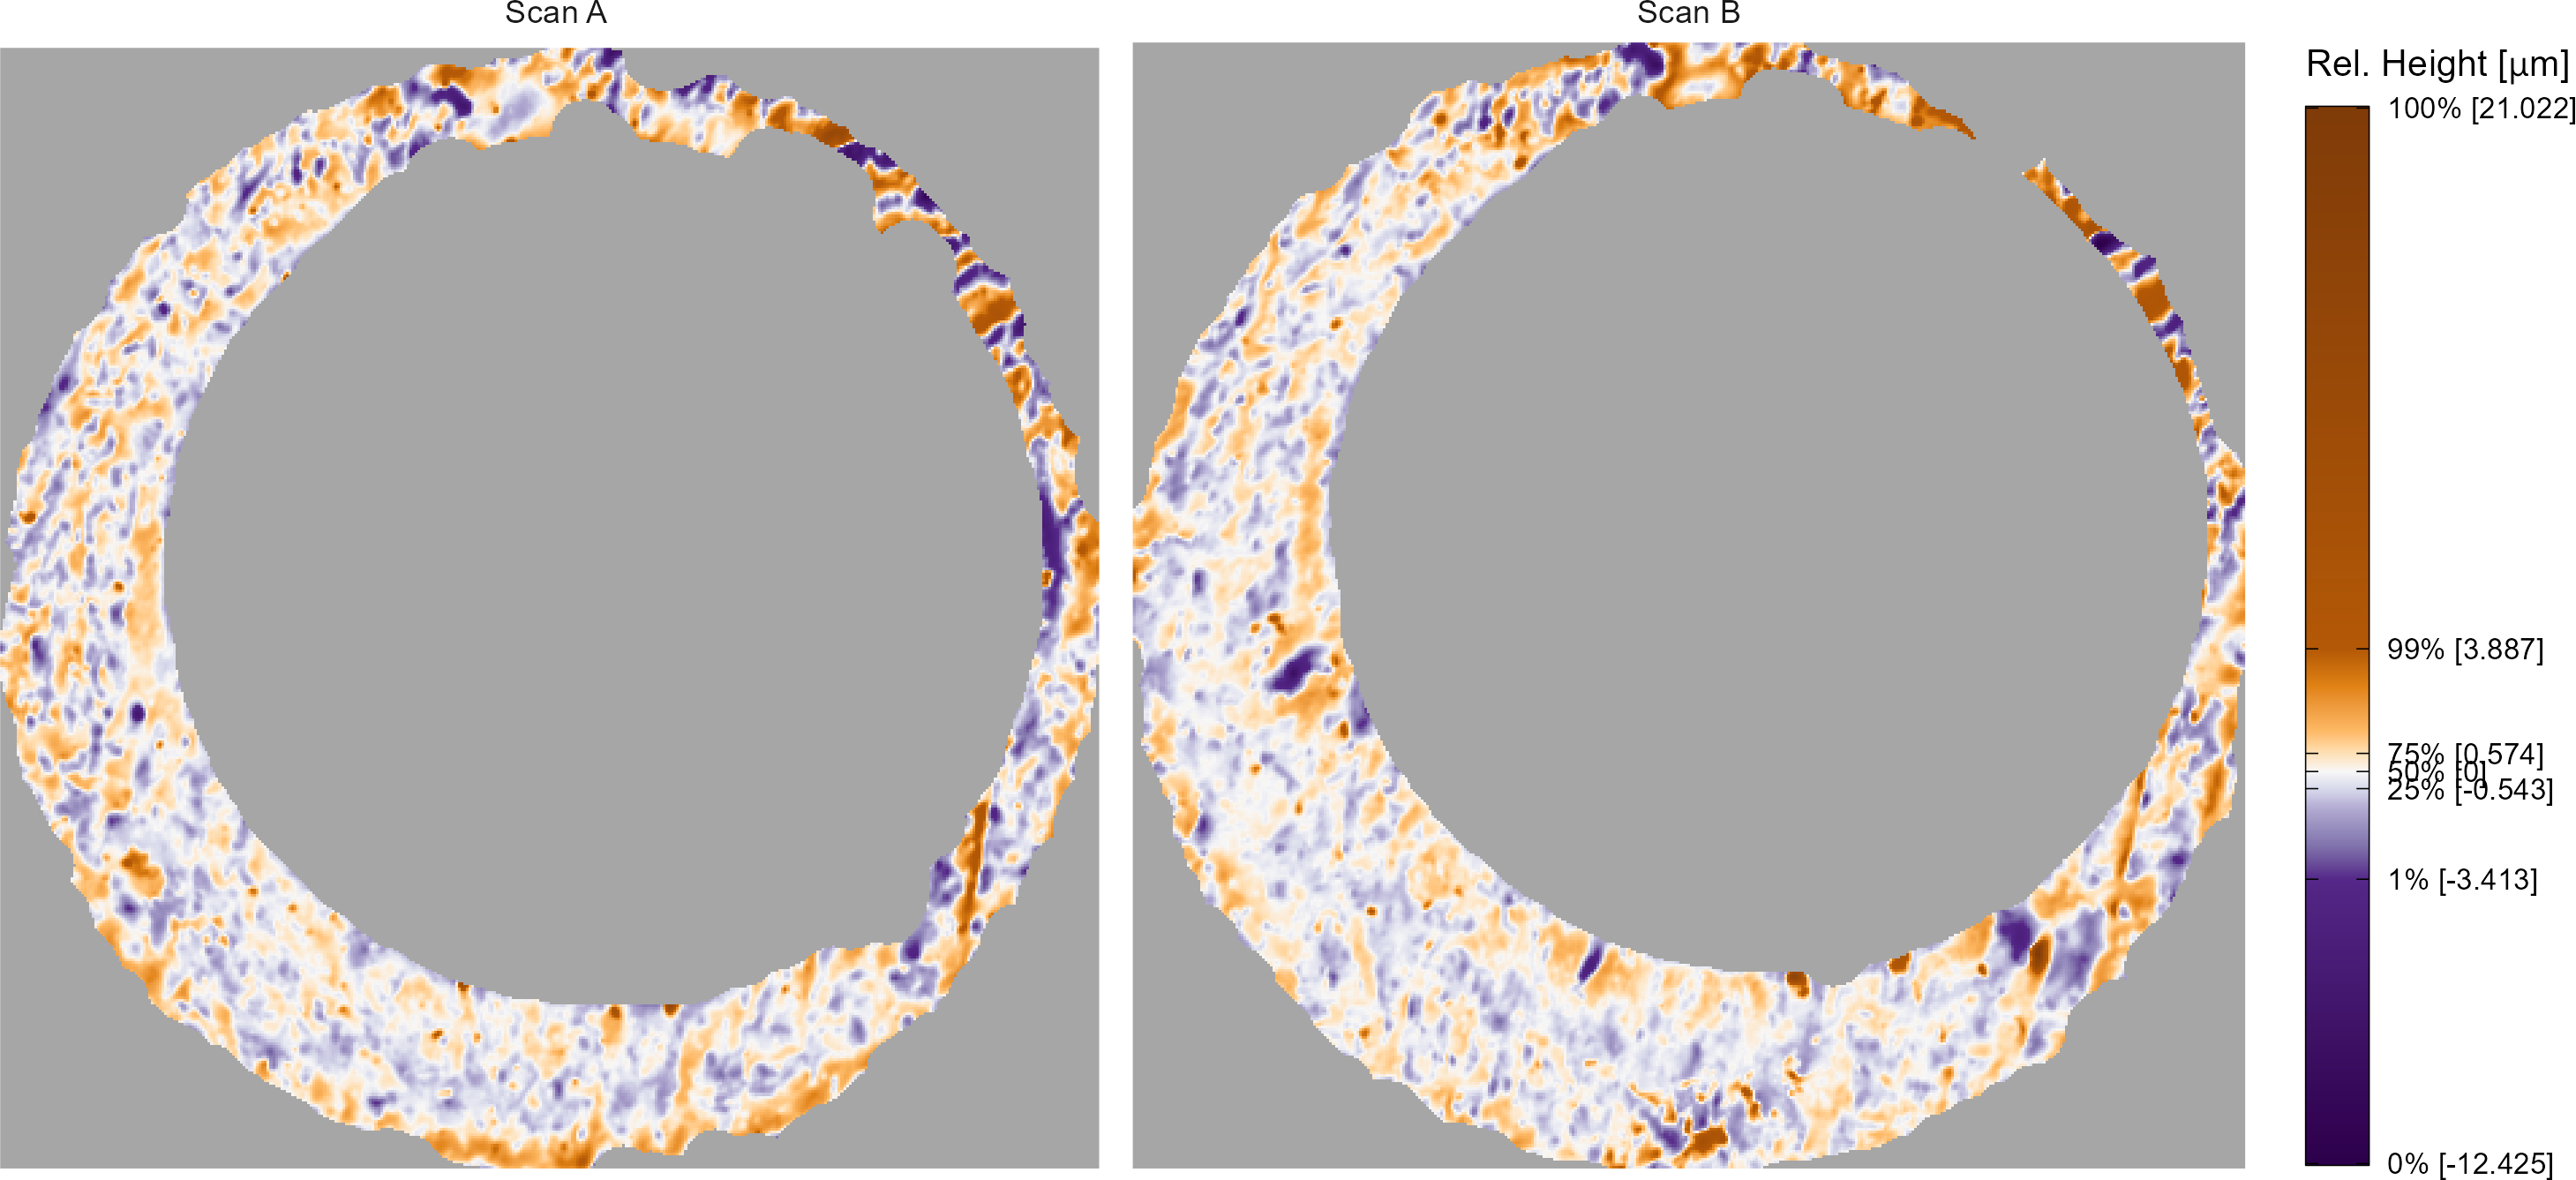
\includegraphics[width=.5\textwidth]{figures/matchPair} \caption{\label{fig:matchPair} A matching pair of processed cartridge case scans. We measure the similarity between these cartridge cases using the distinguishable breech face impressions on their surfaces.}\label{fig:unnamed-chunk-3}
\end{figure}

Note that the calculation of the CCF requires that all missing values,
including structural missing values, are imputed in \(A\) and \(B\). We
impute missing values in a scan with the average non-missing value in
that scan. As a result of imputing a large number of missing values, we
found in our experimentation the estimated registrations
\((\theta^*, m^*, n^*)\) to be reliable but the value of \(CCF_{\max}\)
to not be a reliable measure of similarity for scans. We discuss how we
compute more reliable measures of similarity in
\ref{featureCalculation}.

\hypertarget{full-scan-registration}{%
\subsubsection{Full-Scan Registration}\label{full-scan-registration}}

We first estimate the registration between two full scans \(A\) and
\(B\) using \autoref{alg:registration} with a rotation grid
\(\pmb{\Theta} = \{-30^\circ, -27^\circ,...,27^\circ,30^\circ\}\). This
results in an estimated registration \((m^*,n^*,\theta^*)\) and
similarity measure \(CCF_{\max}\). We also perform
\autoref{alg:registration} with the roles of \(A\) and \(B\) reversed,
meaning the target scan \(A\) is aligned to source scan \(B\).

To accommodate these two comparison directions, we introduce a new
subscript \(d = A,B\), referring to the source scan in
\autoref{alg:registration}. Consequently, we obtain two sets of
estimated registrations, \((m^*_d,n^*_d,\theta^*_d)\) and
\(CCF_{\max,d}\), for
\(d=A,B\).\footnote{In reality, the true aligning registrations in the two comparison directions are opposites of each other. However, because we compare discretely-indexed arrays using a nearest-neighbor interpolation scheme, the estimated registrations may differ slightly.}

\hypertarget{cell-based-registration}{%
\subsubsection{Cell-Based Registration}\label{cell-based-registration}}

We next perform a cell-based comparison procedure, which begins with
selecting one of the matrices, say \(A\), as the ``source'' matrix that
is partitioned into a grid of cells. The left side of
\autoref{fig:cellGridExample} shows an example of such a cell grid
overlaid on a scan. Each of these source cells will be compared to the
``target'' matrix, in this case \(B^*\). Because \(A\) and \(B^*\) are
already partially aligned from the full-scan registration procedure, we
compare each source cell to \(B^*\) using a new rotation grid of
\(\pmb{\Theta}'_A = \{\theta^*_A - 2^\circ, \theta^*_A - 1^\circ,\theta^*_A,\theta^*_A + 1^\circ,\theta^*_A + 2^\circ\}\).

We now extend the surface matrix notation introduced previously to
accommodate cells. Let \(A_{t}\) denote the \(t\)-th cell of matrix
\(A\), \(t = 1,...,T_A\) where \(T_A\) is the total number of cells
containing non-missing values in scan \(A\) (e.g., \(T_A = 43\) in
\autoref{fig:cellGridExample}) and let \((a_t)_{ij}\) denote the
\(i,j\)-th element of \(A_t\). The cell-based comparison procedure is
outlined in \autoref{alg:cellComparison}.

\begin{algorithm}[H]
\KwData{Source matrix $A$, target matrix $B^*$, grid size $R \times C$, and rotation grid $\pmb{\Theta}'_A$}
\KwResult{Estimated translations and $CCF_{\max}$ values per cell, per rotation}
Partition $A$ into a grid of $R \times C$ cells\;
Discard cells containing only missing values, leaving $T_A$ remaining cells\;
\For{$\theta \in \pmb{\Theta}'_A$}{
Rotate $B^*$ by $\theta$ to obtain $B^*_\theta$\;
\For{$t = 1,...,T_A$}{
Calculate $CCF_{\max, A,t,\theta} = \max_{m,n} (a_t \star b^*_\theta)_{mn}$\;
Calculate translation $[m^*_{A,t,\theta},n^*_{A,t,\theta}] = \arg \max_{m,n} (a_t \star b^*_\theta)_{mn}$
}
}
\Return{$\pmb{F}_A = \{(\theta, m^*_{A,t,\theta},n^*_{A,t,\theta}, CCF_{\max,A,t,\theta}) : \theta \in \pmb{\Theta}'_A, t = 1,...,T_A\}$}
\caption{Cell-Based Comparison Procedure}
\label{alg:cellComparison}
\end{algorithm}

We can think of \autoref{alg:registration} as a specific case of
\autoref{alg:cellComparison} where \(R = C = 1\), but we distinguish the
algorithms in this paper based on the intended use of the result. Rather
than exclusively returning the registration that maximizes the overall
CCF as in \autoref{alg:registration}, \autoref{alg:cellComparison}
returns the set \(\pmb{F}_A\) of translations and CCF values for each of
the \(T_A\) cells and each rotation in \(\pmb{\Theta}'_A\).

\begin{figure}[htbp]
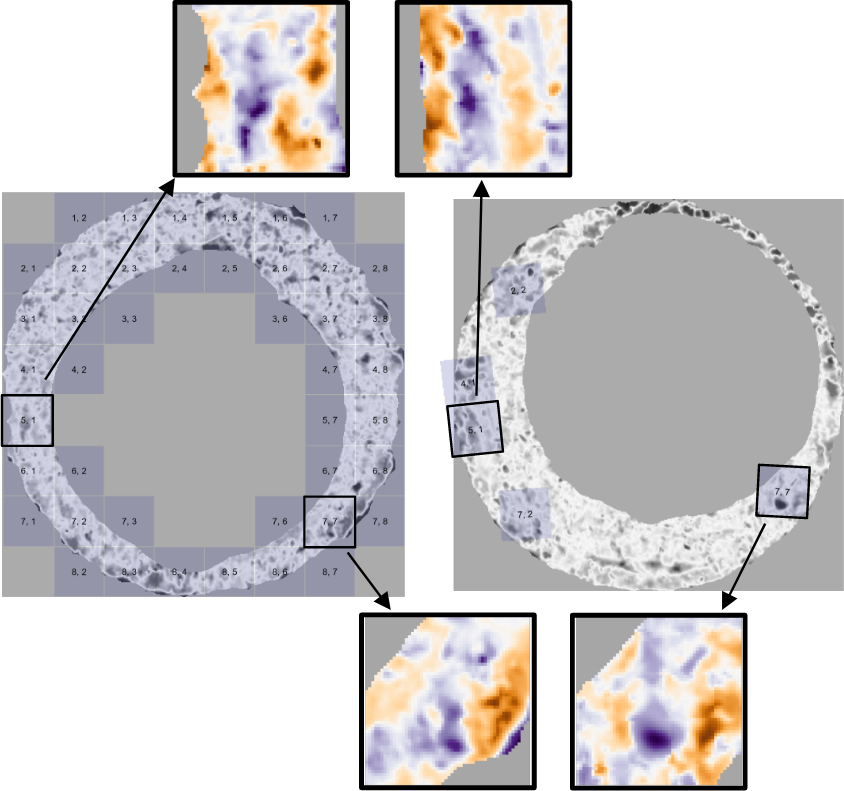
\includegraphics[width=.5\textwidth]{images/cellGridExample_nonMatch} \caption{\label{fig:cellGridExample} Estimated registrations of cells from a non-match pair of cartridge cases. A source scan (left) is separated into an $8 \times 8$ grid of cells. We exclude cells containing only missing values (visualized here as gray pixels). Each source cell is compared to a target scan (right) to estimate where it aligns best. We show a handful of cells at their estimated alignment in the target scan and magnify the surfaces captured by cell pairs 5, 1 and 7, 7. Although the cartridge case pair is non-matching, we note that there are similarities in the surface markings for these cell pairs.}\label{fig:unnamed-chunk-4}
\end{figure}

\autoref{fig:cellGridExample} shows the estimated registrations of cells
between two non-match cartridge cases. We magnify the surface values
captured by cell pairs 5, 1 and 7, 7 and note the similarities in the
surface values; for example, the dark purple region in the middle of the
cell 7, 7 pair.

Next, we introduce a set of similarity features for two cartridge case
scans. We calculate features at two scales: between two full scans and
between individual cells. Analogous to how a forensic examiner uses a
comparison microscope with different magnification levels, this allows
us to assess the similarity between two scans at the macro and micro
levels.

\hypertarget{featureCalculation}{%
\subsection{Feature Calculation}\label{featureCalculation}}

The result of the full scan and cell-based comparisons is a set of
estimated registrations with associated \(CCF_{\max}\) values. We
compute statistics on these results based on how we expect these
registrations to behave for matching vs.~non-matching cartridge case
pairs. Similar to the assumption made in the Congruent Matching Cells
algorithm, we expect that cells will agree on a particular registration
if the two cartridge cases truly match, suggesting that a measure of
spread of the estimated registrations would be an informative statistic.
Further, we would expect that the consensus-estimated registrations
should be approximately opposite across the two comparison directions
(i.e., registering \(A\) to \(B\) is the opposite of registering \(B\)
to \(A\)).

We first introduce a set of \emph{registration-based features} based on
descriptive statistics of the full scan and cell-based registrations.
Then, we discuss a set of \emph{density-based features} based on
applying a density-based clustering algorithm to the cell registrations
\(\pmb{F}_A\) and \(\pmb{F}_B\).

\hypertarget{registration-based-features}{%
\subsubsection{Registration-based
Features}\label{registration-based-features}}

For \(d = A\), we apply the registration transformation
\((m^*_A,n^*_A,\theta^*_A)\) to \(B\) to obtain \(B^*\). Because the
calculation of the \(CCF_{\max}\) requires imputing missing values in
both the source and target scans, we found the \(CCF_{\max}\) values to
not be a reliable measure of similarity for two cartridge cases.
Instead, we compute the \emph{pairwise-complete correlation}, \(cor\),
which is equivalent to the Pearson correlation between the overlapping,
non-missing elements of \(A\) and \(B^*\).

We compute the pairwise-complete correlation between \(A\) and \(B^*\),
resulting in \(cor_{\text{full},A}\). We repeat this in the other
comparison direction to obtain \(cor_{\text{full},B}\) and average the
two:
\(cor_{\text{full}} = \frac{1}{2}\left(cor_{A,\text{full}} + cor_{B,\text{full}}\right)\).
We assume that the \textbf{full-scan pairwise-complete correlation},
\(cor_{\text{full}}\), is large for truly matching cartridge cases.

Just as with the whole-scan registration, we calculate the
pairwise-complete correlation between each cell \(A_t\) and a matrix
\(B_{\theta,t}^*\) of the same size extracted from \(B^*_{\theta}\)
after translating by \([m^*_{A,\theta},n^*_{A,\theta}]\). From this we
obtain a set of pairwise-complete correlations for each cell and
rotation:
\(\{cor_{A,t,\theta} : t = 1,...,T_A, \theta \in \pmb{\Theta}'_A\}\).

We repeat \autoref{alg:cellComparison} and the pairwise-complete
correlation calculation using \(B\) as the source scan and \(A^*\) as
the target, resulting in cell-based registration set \(\pmb{F}_B\) and
pairwise-complete correlations
\(\{cor_{B,t,\theta} : t = 1,...,T_B, \theta \in \pmb{\Theta}'_B\}\).

For \(d = A,B\) and \(t = 1,...,T_d\), define the cell-wise maximum
pairwise-complete correlation as:

\[
cor_{d,t} = \max_{\theta} \{cor_{d,t,\theta} : \theta \in \pmb{\Theta}'_d\}.
\]

We compute two features, the \textbf{average} and \textbf{standard
deviation of the cell-based pairwise-complete correlations}, using the
correlation data:

\begin{align*}
\overline{cor}_{\text{cell}} &= \frac{1}{T_A + T_B} \sum_{d \in \{A,B\}} \sum_{t=1}^{T_d} cor_{d,t} \\
s_{cor} &= \sqrt{\frac{1}{T_A + T_B - 1} \sum_{d \in \{A,B\}} \sum_{t=1}^{T_d} (cor_{d,t} - \overline{cor}_{\text{cell}})^2}.
\end{align*}

We expect \(\overline{cor}_{\text{cell}}\) and \(s_{cor}\) to be large
for truly matching cartridge case pairs relative to non-matching pairs.

For \(d = A,B\) and \(t = 1,...,T_d\), define the per-cell estimated
translations and rotation as:

\begin{align*}
\theta^*_{d,t} &= \arg \max_{\theta} \{CCF_{\max,d,t,\theta} : \theta \in \pmb{\Theta}'_d\} \\
m^*_{d,t} &= m^*_{\theta^*_{d,t},d,t} \\
n^*_{d,t} &= n^*_{\theta^*_{d,t},d,t}.
\end{align*}

We compute the \textbf{standard deviation of the cell-based estimated
registrations} using the estimated translations and rotations:

\begin{align*}
s_{\theta^*} =  \sqrt{\frac{1}{T_A + T_B - 1} \sum_{d \in \{A,B\}} \sum_{t=1}^{T_d} (\theta^*_{d,t} - \bar{\theta}^*)^2} \\
s_{m^*} =  \sqrt{\frac{1}{T_A + T_B - 1} \sum_{d \in \{A,B\}} \sum_{t=1}^{T_d} (m^*_{d,t} - \bar{m}^*)^2} \\
s_{n^*} = \sqrt{\frac{1}{T_A + T_B - 1} \sum_{d \in \{A,B\}} \sum_{t=1}^{T_d} (n^*_{d,t} - \bar{n}^*)^2}
\end{align*}

where

\begin{align*}
\bar{m}^* &= \frac{1}{T_A + T_B} \sum_{d \in \{A,B\}}\sum_{t=1}^{T_d} m^*_{d,t} \\
\bar{n}^* &= \frac{1}{T_A + T_B} \sum_{d \in \{A,B\}} \sum_{t=1}^{T_d} n^*_{d,t} \\
\bar{\theta}^* &= \frac{1}{T_A + T_B} \sum_{d \in \{A,B\}} \sum_{t=1}^{T_d} \theta^*_{d,t}.
\end{align*}

We expect \(s_{\theta^*}, s_{m^*},s_{n^*}\) to be small for truly
matching cartridge case pairs relative to non-matching pairs.

From the full-scan and cell-based registration procedures, we obtain six
features summarized in \autoref{tab:registrationFeatures}.

\begin{table}[htbp]
\centering
\begin{tabular}{p{.11\linewidth} p{.7\linewidth}}
$cor_{\text{full}}$ & Full-scan pairwise-complete correlation \\
$\overline{cor}_{\text{cell}}$ & Average cell-based pairwise-complete correlation \\
$s_{cor}$ & Standard deviation of the cell-based pairwise-complete correlations \\
$s_{m^*}$ & Standard deviation of the cell-based vertical translations (in microns) \\
$s_{n^*}$ & Standard deviation of the cell-based horizontal translations (in microns) \\
$s_{\theta^*}$ & Standard deviation of the cell-based rotations (degrees)
\end{tabular}
\caption{Six similarity features based on registering full scans and cells.}
\label{tab:registrationFeatures}
\end{table}

\hypertarget{density-based-features}{%
\subsubsection{Density-Based Features}\label{density-based-features}}

We wish to identify when multiple cells agree on, or cluster around, a
particular registration value. However, pursuant with the notion that
only certain regions of matching cartridge cases contain distinctive
markings, it is unreasonable to assume and empirically rare that
\textbf{all} cells agree on a single registration. In fact, it is common
for many cells to disagree on a registration. For example, the left
scatterplot in \autoref{fig:dbscanScatterplot} shows the per-cell
estimated translations \([m^*_{A,t,\theta}, n^*_{A,t,\theta}]\) when
scan \(A\) is used as source and \(B^*\) as target rotated by
\(\theta = 3^\circ\). The right scatterplot shows the per-cell estimated
translations with the roles of \(A\) and \(B^*\) reversed for
\(\theta = -3^\circ\). We see distinctive clusters, the black points, in
both plots among many noisy, gray points. The task is to isolate the
clusters among such noise.

We use the Density-Based Spatial Clustering of Applications with Noise
(DBSCAN) algorithm proposed by \citet{Ester1996} to identify clusters.
Compared to other clustering algorithms such as k-means
\citep{MacQueen1967}, DBSCAN does not require a pre-defined number of
expected clusters. Instead, the algorithm forms clusters if the number
of points within an \(\epsilon > 0\) distance of a point exceeds some
pre-defined threshold, \(minPts > 1\). If a point does not belong to a
cluster, then DBSCAN labels that point as ``noise.''

In \autoref{fig:dbscanScatterplot}, we use a \(4 \times 4\) grid of
cells to which we apply DBSCAN with \(\epsilon = 3\) and \(minPts = 3\).
The resulting clusters for the two comparison directions are 7 and 9
cells, respectively, visualized in \autoref{fig:dbscanScatterplot} as
black points. This indicates that about half of the cells in the
\(4 \times 4\) grid agree on a registration in both comparison
directions. Additionally, the mean cluster centers are approximately
close to 0:
\((\hat{m}_A,\hat{n}_A,\hat{\theta}_A) \approx (0.29, 0.57, 0^\circ)\)
when \(A\) is used as source compared to
\((\hat{m}_B,\hat{n}_B,\hat{\theta}_B) \approx (-0.67, 0, 0^\circ)\)
when \(B^*\) is used as source. If \(A\) and \(B\) were truly matching
and the full scan registration from \autoref{alg:registration}
successfully aligned the two scans, then we wouldn't expect the cells to
move much in their respective registrations, which is illustrated in
this example. For non-matching scans, we wouldn't expect the cell
registrations to agree only by coincidence.

\begin{figure}[htbp]
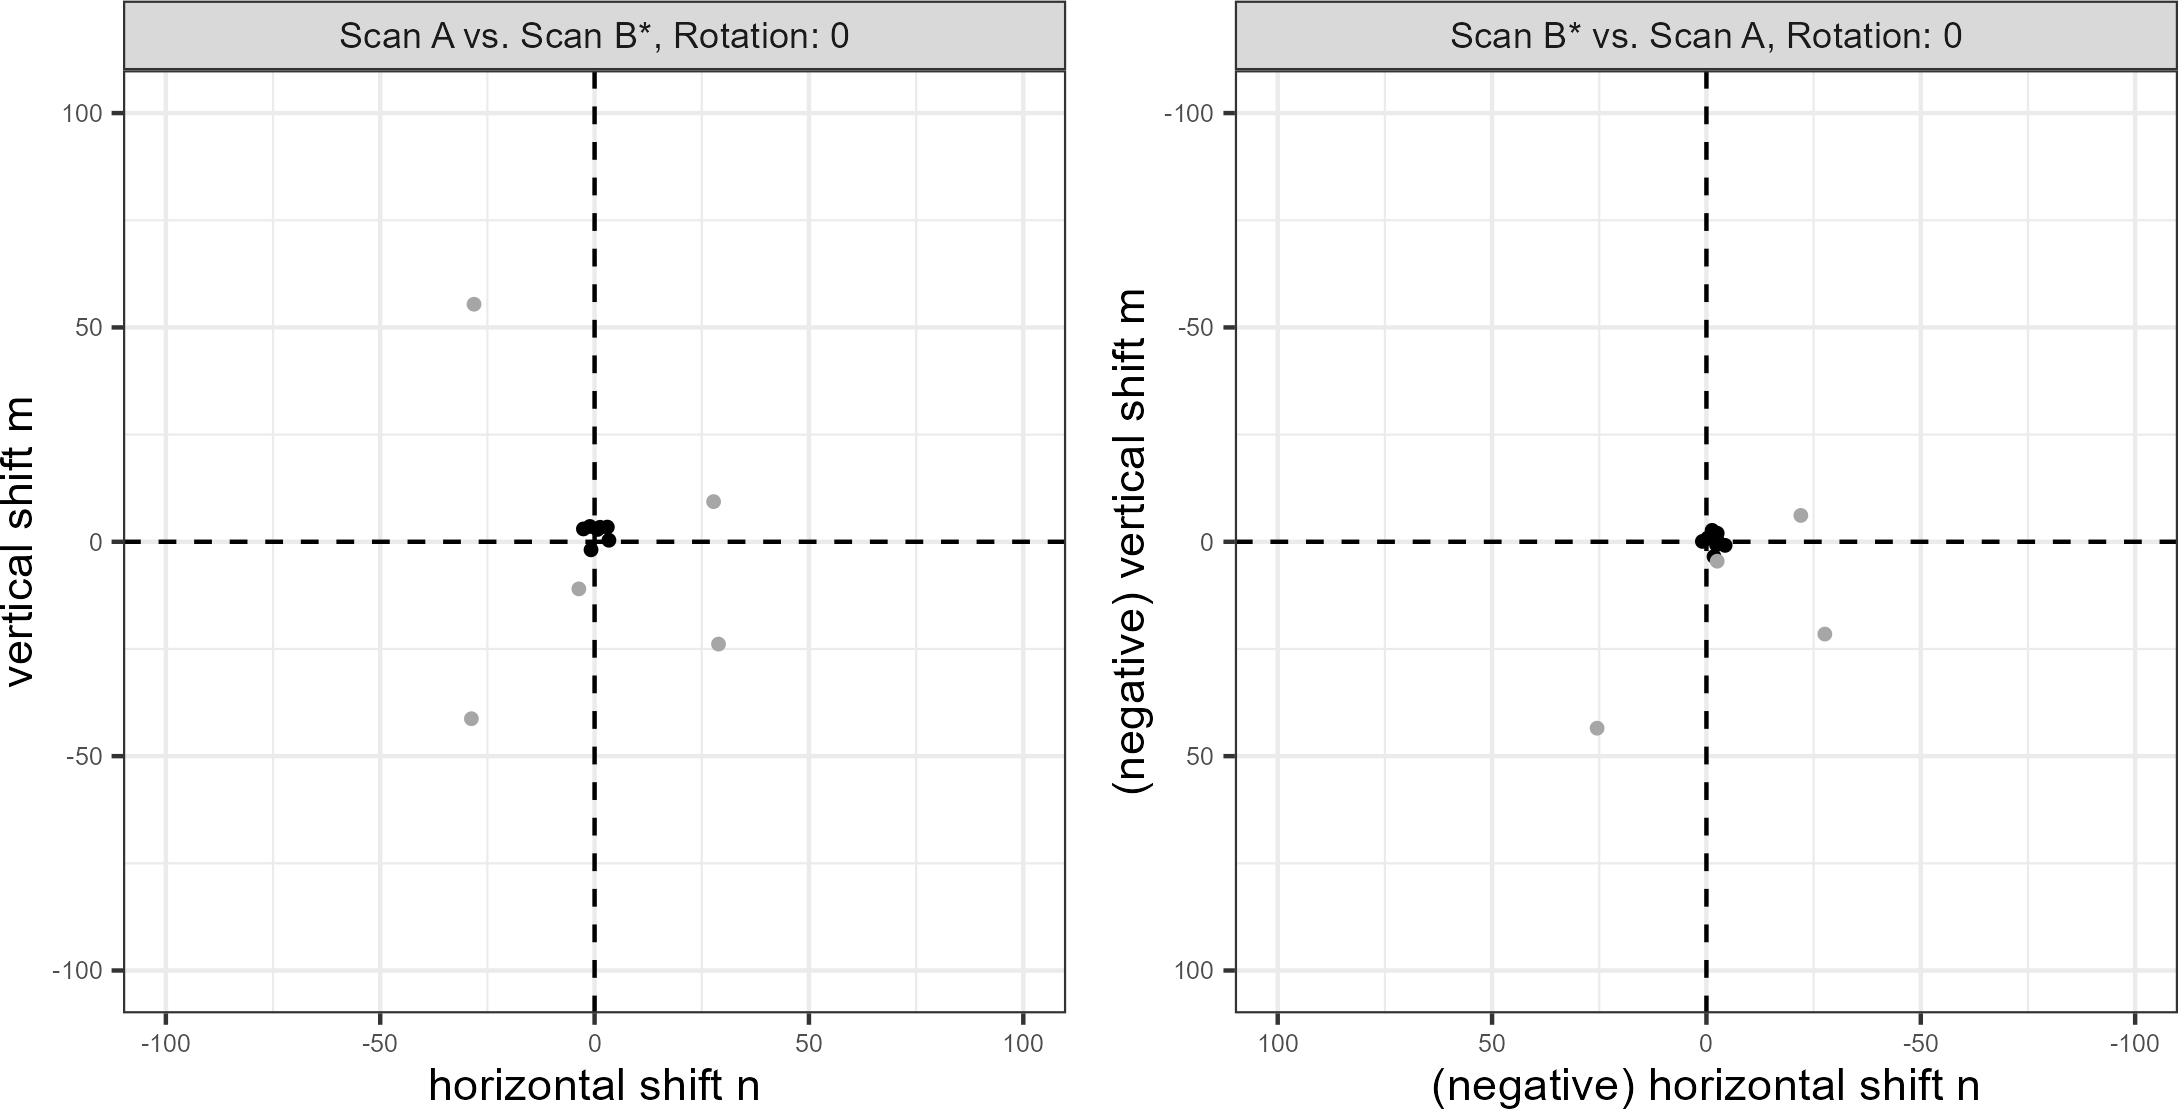
\includegraphics[width=.5\textwidth]{figures/dbscanScatterplot} \caption{\label{fig:dbscanScatterplot} Cluster assignments based on the Density Based Spatial Clustering with Applications to Noise (DBSCAN) algorithm for estimated translations in two comparison directions. Using scan $A$ as source results in a cluster of size 14 (left) compared to 13 when scan $B^*$ is used as source (right). Noting the reversed axes in the right plot, we see that the clusters are located approximately opposite of each other. Points are jittered for visibility.}\label{fig:unnamed-chunk-7}
\end{figure}

To calculate the density-based features, we first use a 2D kernel
density estimator \citep{MASS} to identify the rotation
\(\hat{\theta}_d\) at which the per-cell translations achieve the
highest density. Next, we compute clusters using the DBSCAN algorithm
amongst the estimated translations
\(\{(m^*_{d,t,\hat{\theta}_d},n^*_{d,t,\hat{\theta}_d}) : t = 1,...,T_d\}\)
like those shown in \autoref{fig:dbscanScatterplot}.\footnote{If more
  than one cluster is identified, we binarize the points based on
  whether they were assigned to any cluster or if they are a noise point
  and proceed as if there is only one cluster. We assume that two or
  more clusters form only because of the course rotation grid
  considered. Were a finer grid used, the points would coalesce into a
  single cluster around the true translation value. This assumption has
  empirical support through our experimentation.} Let \(\pmb{C}_d\)
denote the set of cells in the DBSCAN cluster. We treat the mean cluster
centers as the estimated translations \([\hat{m}_d,\hat{n}_d]\).

We calculate four features from the density-based clustering procedure:
\textbf{average DBSCAN cluster size} \(C\), the \textbf{DBSCAN cluster
indicator} \(C_0\), and the \textbf{root sum of squares of the
dens}ity-estimated registrations
\((\Delta_\theta, \Delta_{\text{trans}})\) defined as:

\begin{align*}
C &= \frac{1}{2}\left(|\pmb{C}_A| + |\pmb{C}_B|\right) \\
C_0 &= I(|\pmb{C}_A| > 0 \text{ and } |\pmb{C}_B| > 0)\\
\Delta_\theta &= |\hat{\theta}_A + \hat{\theta}_B| \\
\Delta_{\text{trans}} &= \sqrt{(\hat{m}_A + \hat{m}_B)^2 + (\hat{n}_A + \hat{n}_B)^2}
\end{align*} where \(|\pmb{C}_d|\) denotes the cardinality of
\(\pmb{C}_d\) and \(I(\cdot)\) is the identity function equal to 1 if
the predicate argument ``\(\cdot\)'' evaluates to TRUE and 0 otherwise.
We use both \(C\) and \(C_0\) because of potential missingness in the
values of \(C\) if no cluster is identified. Missing \(C\) values are
imputed using the median non-missing value when fitting classifiers, so
the missingness information is retained in \(C_0\).

For truly matching cartridge case pairs, we expect \(C\) to be large and
\(\Delta_\theta, \Delta_{\text{trans}}\) to be small relative to
non-matching pairs and for \(C_0\) to be equal to 1. We obtain four
density-based features summarized in \autoref{tab:dbscanFeatures}.

\begin{table}[htbp]
\centering
\begin{tabular}{p{.11\linewidth} p{.7\linewidth}}
$C$ & Average DBSCAN cluster size \\
$C_0$ & DBSCAN cluster indicator \\
$\Delta_\theta$ & Absolute sum of the density-estimated rotations (degrees) \\
$\Delta_{\text{trans}}$ & Root sum of squares of the density-estimated translations (in microns)
\end{tabular}
\caption{Four similarity features based on the density-based clustering procedure.}
\label{tab:dbscanFeatures}
\end{table}

\hypertarget{model-fitting}{%
\subsection{Model Fitting}\label{model-fitting}}

Cross-validation procedure

\hypertarget{results}{%
\section{Results}\label{results}}

\hypertarget{discussion}{%
\section{Discussion}\label{discussion}}

\hypertarget{conclusion}{%
\section{Conclusion}\label{conclusion}}

\begin{acknowledgments}
This work was partially funded by the Center for Statistics and
Applications in Forensic Evidence (CSAFE) through Cooperative Agreement
70NANB20H019 between NIST and Iowa State University, which includes
activities carried out at Carnegie Mellon University, Duke University,
University of California Irvine, University of Virginia, West Virginia
University, University of Pennsylvania, Swarthmore College and
University of Nebraska, Lincoln.

We would like to thank the technicians and staff at the Roy J. Carver
High Resolution Microscopy Facility for collecting the topographical
scans used in this paper.

\end{acknowledgments}

\begin{appendices}

\section{Congruent Matching Cells Algorithm Criteria} \label{appendixCMC}

This section will provide a more thorough definition of the classification criteria used in the Congruent Matching Cells algorithm as proposed in \citet{song_proposed_2013}.
This section assumes that the reader is familiar with the notation and algorithms, \autoref{alg:registration} and \autoref{alg:cellComparison}, introduced in \ref{methods}.

\end{appendices}

% -------------------------------------------------------------------------------------------------------------------
%   Appendix  (optional)

%\appendix
%\section{Appendix title}

%If only one appendix, please use
%\appendix*
%\section{Appendix title}


%=======================================================

%Use \bibliography{<name of your .bib file>}+
%to make your bibliography with BibTeX.

%=======================================================

\bibliography{biblio.bib}


\end{document}
